	\centering
	\begin{subfigure}{0.48\textwidth}
		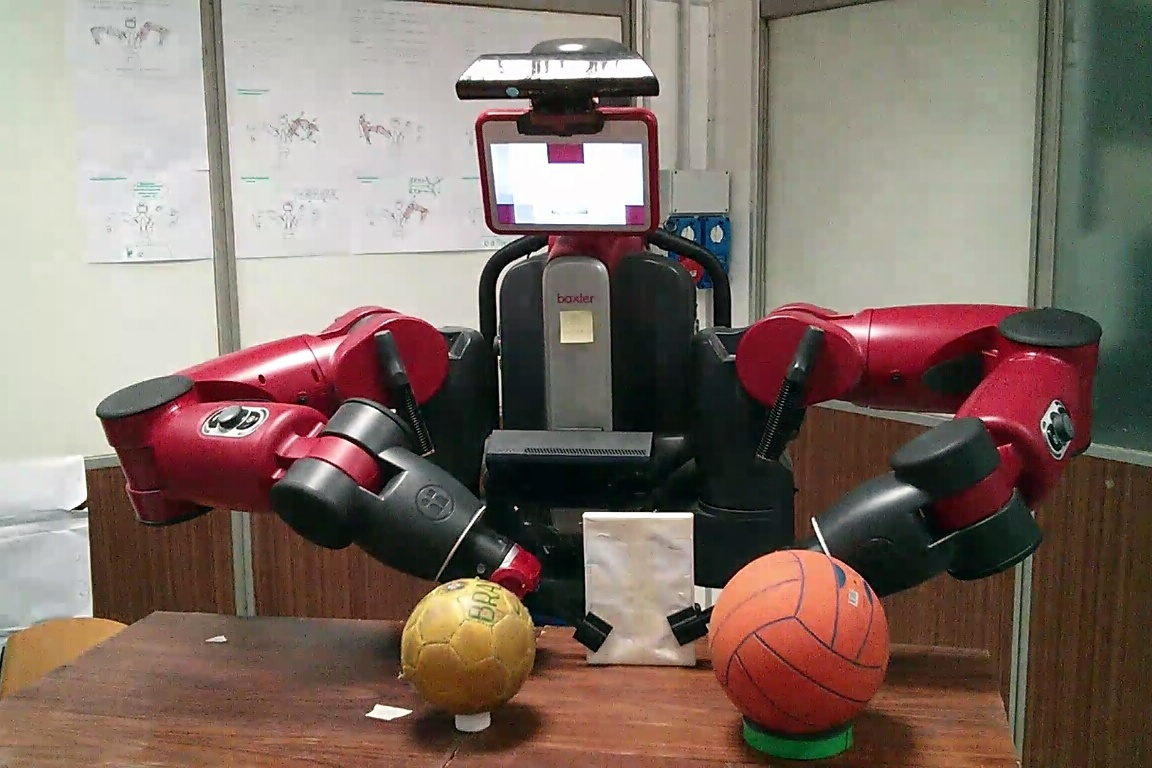
\includegraphics[width=\textwidth]{singleAgent/vidFrame1.jpeg}%
		\caption{}
		\label{fig:vidFrame1}	
	\end{subfigure}
    \hfill
	\begin{subfigure}{0.48\textwidth}
		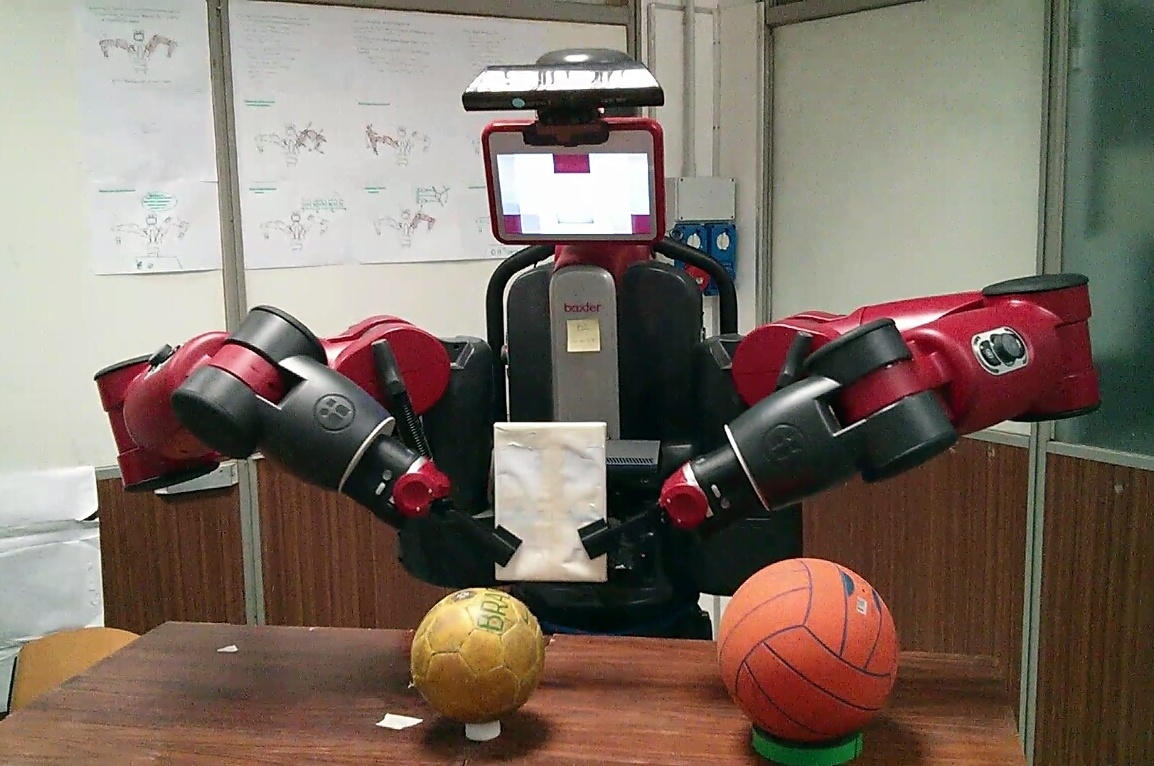
\includegraphics[width=\textwidth]{singleAgent/vidFrame2.jpeg}%
		\caption{}
		\label{fig:vidFrame2}	
	\end{subfigure}
	\vspace{0.2cm}
	\begin{subfigure}{0.48\textwidth}
		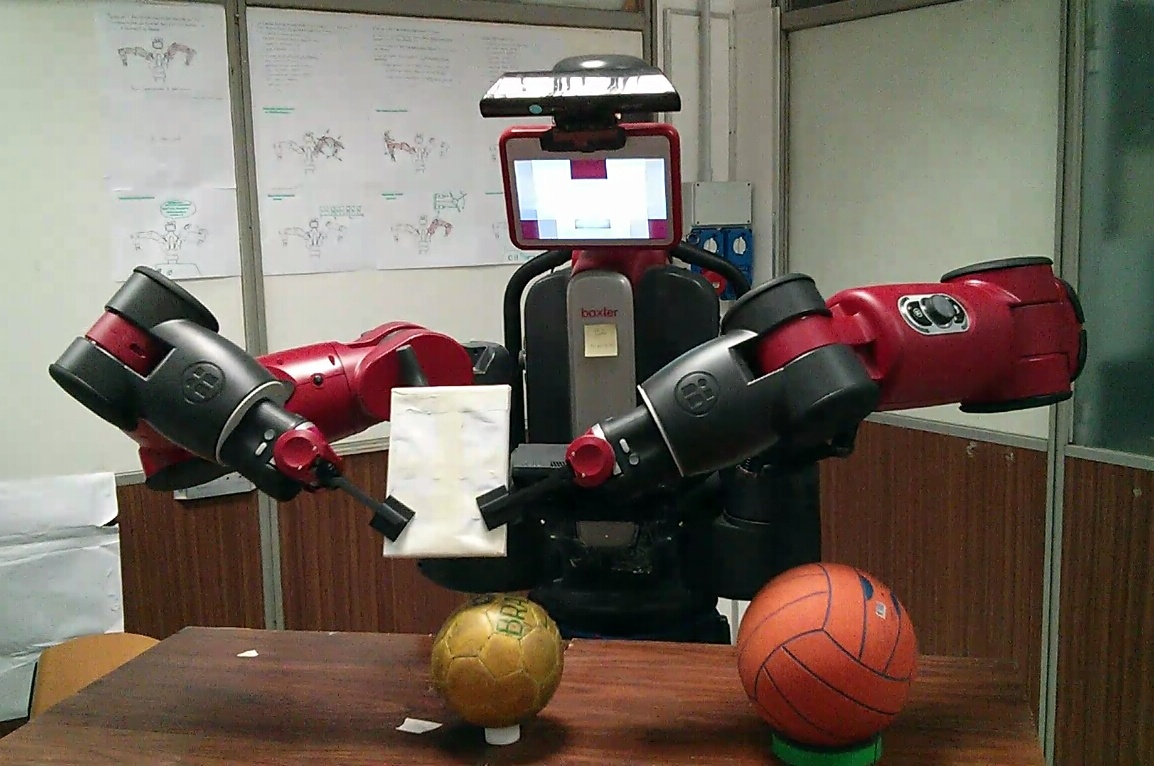
\includegraphics[width=\textwidth]{singleAgent/vidFrame3.jpeg}%
		\caption{}
		\label{fig:vidFrame3}	
	\end{subfigure}
    \hfill
    \begin{subfigure}{0.48\textwidth}
		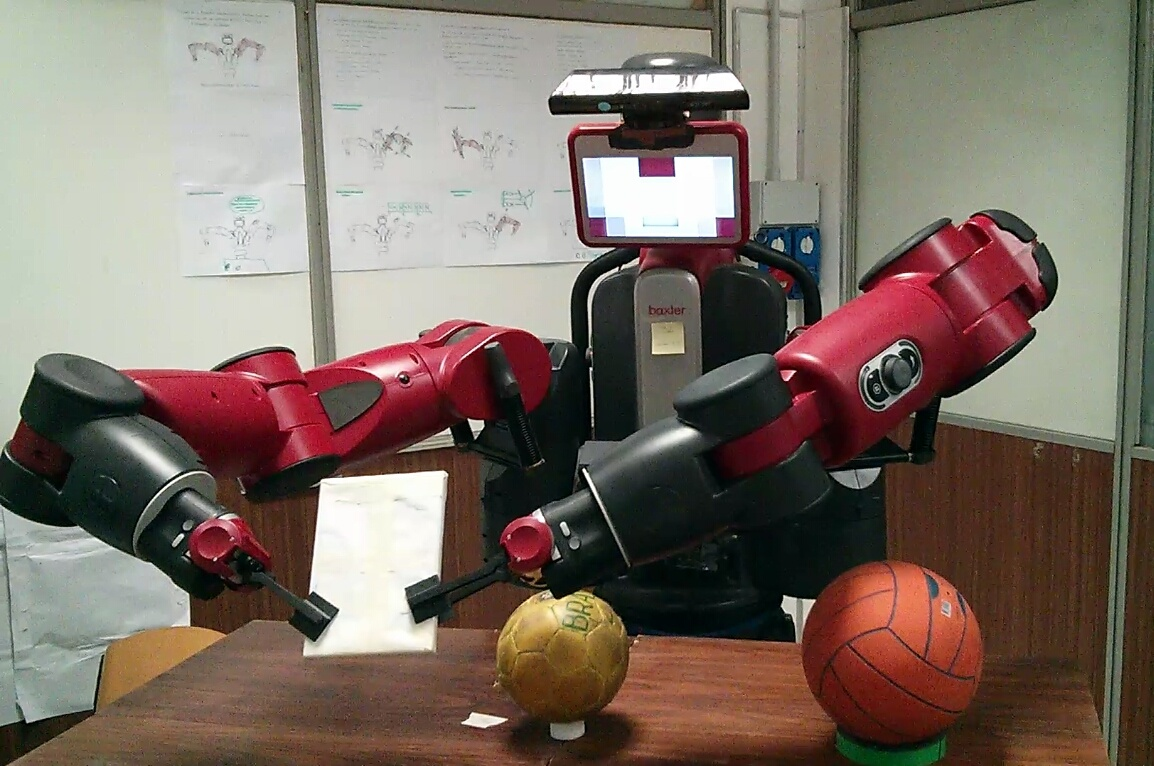
\includegraphics[width=\textwidth]{singleAgent/vidFrame4.jpeg}%
		\caption{}
		\label{fig:vidFrame4}
	\end{subfigure}
\caption{A series of successive still frames from one of the coordinated transportation experiments. As it can be seen in the last two frames \ref{fig:vidFrame3} and \ref{fig:vidFrame4}, the elbow is gradually raising its height to stay out of the bounding box defined for the obstacle.}

